\section{Manual para el desarrollador}

El usuario final de MindMapJS puede tanto un programador, como un usuario final. Para los primeros se ha elaborado el siguiente documento, buscando facilitar su integración en otros proyectos. 

\subsection{Dependencias}
Para poder poner en marcha el proyecto debes tener instalado en tu sistema:
\begin{itemize}
\item \textbf{Git}
\item \textbf{NodeJS}
\item \textbf{NPM} en el caso de que no venga integrado con NodeJS. En las últimas versiones NPM ya viene integrado en el instalador de NodeJS. 
\end{itemize}

\subsection{Clonar el MindMapJS}
primero que debemos realizar para poder obtener el código fuente es clonar el proyecto. Para ello, supongo que se tiene ya instalado el Git. Para clonar el proyecto MindMapJS ejecutamos el siguiente comando.

\begin{lstlisting}[language=bash, numbers=left]
$ git clone https://github.com/joseluismolinasoria/MindMapJS.git
\end{lstlisting}

\begin{figure}[tbph]
\centering
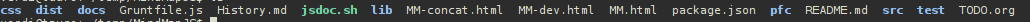
\includegraphics[width=\linewidth]{imagenes/directorioProyecto}
\caption{Estructura de directorios de MindMapJS}
\label{fig:directorio-proyecto}
\end{figure}

En la estructura del proyecto \ref{fig:directorio-proyecto} podemos observar como disponemos de los siguientes directorios:
\begin{itemize}
\item Directorio \textbf{css} con los ficheros de estilo de la página/s HTML.
\item Directorio \textbf{dist} dónde se generará las versiones de distribución de la librería Javascripts de MindMapJS.
\item Directorio \textbf{docs} con la documentación, en formato HTML, del API de MindMapJS. 
\item Directorio \textbf{lib} con librerías externas al proyecto como KineticJS.
\item Directorio \textbf{pfc} este documento.
\item Directorio \textbf{src} con todo el código fuente Javascripts del proyecto.
\item Directorio \textbf{test} con los fuentes de los test unitarios de MindMapJS.
\item Y en general ficheros de configuración y páginas HTML de demos, como un fichero TODO en formato Org-mode.
\end{itemize}


\subsection{Resolver dependencias}

El siguiente paso es tener en cuenta es la resolución de dependencias. Para ello, haremos uso de NPM. Para este paso debes tener NodeJS y NPM. El siguiente comando nos descargará las librerías y herramientas necesarias para el desarrollo.

\begin{lstlisting}[language=bash, numbers=left]
$ npm install
\end{lstlisting}

Ahora ya tenemos el proyecto operativo para realizar nuestras mejoras.

\subsection{Construir la versión de desarrollo}
Para obtener una versión de desarrollo de la librería utilizaremos el siguiente comando.

\begin{lstlisting}[language=bash, numbers=left]
$ grunt dev
\end{lstlisting}

\begin{figure}[tbph]
\centering
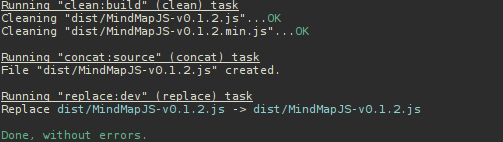
\includegraphics[width=0.6\linewidth]{imagenes/grunt-dev}
\caption{Resultado de ejecutar el comando 'grunt dev'}
\label{fig:grunt-dev}
\end{figure}


Con el obtendremos una concatenación de todos los módulos y clases de MindMapJS. El fichero final es \textbf{dist/MindMapJS-vXXX.js} donde XXX es la versión actual del proyecto.

\subsection{Construir la versión de producción}
Para obtener una versión de producción de MindMapJS utilizaremos el siguiente comando.

\begin{lstlisting}[language=bash, numbers=left]
$ grunt full
\end{lstlisting}

\begin{figure}[tbph]
\centering
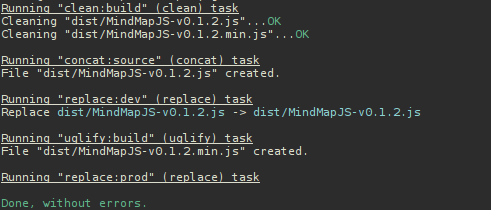
\includegraphics[width=0.5\linewidth]{imagenes/grunt-full}
\caption{Resultado de ejecutar el comando 'grunt full'}
\label{fig:grunt-full}
\end{figure}


Con el obtendremos una concatenación de todos los módulos y clases de MindMapJS. El fichero final es \textbf{dist/MindMapJS-vXXX.min.js} donde XXX es la versión actual del proyecto.

\subsection {JSHint. Verificar el código.}
Para comprobar la validez del código fuente con JSHint, realizaremos:

\begin{lstlisting}[language=bash, numbers=left]
$ grunt hint
\end{lstlisting}

\begin{figure}[tbph]
\centering
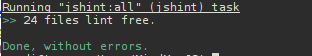
\includegraphics[width=0.5\linewidth]{imagenes/grunt-hint}
\caption{Resultado de ejecutar el comando 'grunt hint'}
\label{fig:grunt-hint}
\end{figure}

\subsection{Tests.}
El siguiente comando lanza la batería de pruebas del proyecto.

\begin{lstlisting}[language=bash, numbers=left]
$ grunt test
\end{lstlisting}

\begin{figure}[tbph]
\centering
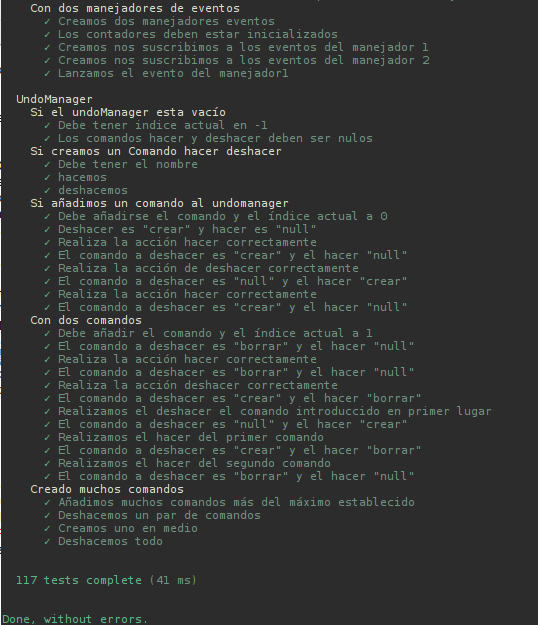
\includegraphics[width=0.5\linewidth]{imagenes/grunt-test}
\caption{Resultado de ejecutar el comando 'grunt test'}
\label{fig:grunt-test}
\end{figure}


\subsection{Generar la documentación del API}

Si es necesario podemos generar API en formato JSDoc. 

\begin{lstlisting}[language=bash, numbers=left]
$ ./jsdocs.sh 
\end{lstlisting}
